
\section{In-Place Test-Time Training}
\label{sec:method-inplace-ttt}

To satisfy the desiderata outlined in \cref{sec:preliminary}, we introduce \textit{\textbf{In-Place} \textbf{T}est-\textbf{T}ime \textbf{T}raining \textbf{(In-Place TTT)}}, a framework designed to unlock TTT capabilities for LLMs. We first present our overall framework, which resolves architectural incompatibility via an in-place design that repurposes existing MLP blocks, while ensuring computational efficiency with a chunk-wise update mechanism (\cref{sec:inplace_ttt_framework}). We then detail our novel LM-aligned objective, which is explicitly designed for LLMs by aligning with the Next-Token Prediction (NTP) goal (\cref{sec:value_and_loss}). Following this, we provide a theoretical analysis of our objective's superior properties (\cref{sec:theory}) and conclude with practical implementation details (\cref{sec:implement}).

\subsection{Overall Framework}
\label{sec:inplace_ttt_framework}

\textbf{Repurposing MLP Blocks for In-Place Adaptation.} 
Previous TTT research has largely positioned it as a potential solution to replace the attention mechanism. However, these prior studies were typically conducted at moderate scales, a regime vastly different from that of modern, billion-parameter LLMs. Consequently, replacing the core attention mechanism—whose learned properties are critical to an LLM's capabilities—is a high-risk architectural modification. Moreover, introducing any new, randomly-initialized layer also creates a conflict with the billions of trained parameters of LLMs, necessitating costly and often impractical retraining to resolve this imbalance.

Our core insight is to sidestep these challenges entirely. Instead of replacing or adding components, we repurpose a ubiquitous module--the Multi-Layer Perceptron (MLP) block--to also serve as the fast weights. Recalling the TTT formulations in \cref{sec:preliminary}, there exist no constraints on the choice of fast weights, i.e., any parameters can serve as fast weights updated via the TTT mechanism. In particular, the MLP blocks in Transformers can also be viewed as a form of key-value memory~\citep{geva2020transformer}, functioning as a ``slow weights" for the vast, general knowledge acquired during pre-training. It is therefore a natural extension to leverage this same component to also function as the adaptive "fast weights", dynamically internalizing transient, in-context information at inference time.

Formally, we adapt the widely used gated MLP architecture~\citep{grattafiori2024llama,yang2025qwen3}. Given the hidden representation $\mathbf{H}$, the gated MLP computes its output representation $\mathbf{O}=\left(\phi(\mathbf{H}\mathbf{W}_{\mathrm{gate}}^\top)\odot(\mathbf{H}\mathbf{W}_{\mathrm{up}}^\top)\right)\mathbf{W}_{\mathrm{down}}^\top$. In our framework, we treat the input projections $\mathbf{W}_{\mathrm{up}}$ and $\mathbf{W}_{\mathrm{gate}}$ as frozen slow weights, while repurposing the final projection matrix, $\mathbf{W}_{\mathrm{down}}$, as the adaptable fast weights. By exclusively updating $\mathbf{W}_{\mathrm{down}}$ in-place, we preserve the model's architectural integrity, transforming TTT from a disruptive restructuring into a lightweight, ``drop-in" enhancement for LLMs. 

\textbf{Efficient Adaptation with Chunk-Wise Updates.} 
Beyond architectural compatibility, our in-place design also unlocks significant computational efficiencies. Conventional TTT methods, by aiming to replace the attention mechanism, were bound to inefficient per-token updates to enforce strict causality and perform fine-grained token mixing. Chunk-wise updating approaches have been explored by recent works to achieve acceleration ~\citep{li2025tnt,sun2023retentive,behrouz2024titans,irie2025fastweightprogramminglinear}. Our framework also follows to sidestep the trade-off entirely. Since we only adapt the MLP blocks and leave the attention layers intact, we are liberated from the per-token constraint, enabling a far more efficient chunk-wise update strategy which further bypasses the small chunk constraints (our ablation study results (Section \ref{sec:exp_ablation}) also verify that our framework is naturally well-suited for chunk-wise—and specifically large chunk-wise—updates, achieving optimal performance with chunk sizes of 512 to 1024).

The process operates as follows. Given the intermediate activations $\mathbf{Z}=\phi(\mathbf{H}\mathbf{W}_{\mathrm{gate}}^\top)\odot(\mathbf{H}\mathbf{W}_{\mathrm{up}}^\top)\in\mathbb{R}^{n\times d_{\mathrm{ff}}}$ and corresponding value targets and outputs $\mathbf{V},\mathbf{O}\in\mathbb{R}^{n\times d_{\mathrm{model}}}$, we partition them into $k$ non-overlapping chunks of size $C$, denoted $\mathbf{\square}_{[i]}=\mathbf{\square}_{iC+1:(i+1)C}\in\mathbb{R}^{C\times d'}$ for $\square\in\{\mathbf{Z},\mathbf{V},\mathbf{O}\}, i\in[k]$ and $d'$ being their corresponding dimension. Let $\mathbf{W}_{\mathrm{down}}^{(i)}$ be the fast weights state before processing chunk $i$ and $\mathbf{W}_{\mathrm{down}}^{(0)}=\mathbf{W}_{\mathrm{down}}$. For each chunk $i\in[k]$, we perform two sequential operations:

\begin{enumerate}
\setlength\itemsep{2pt}
    \item \textbf{Apply Operation:} The current state of the fast weights $\mathbf{W}_{\mathrm{down}}^{(i)}$ are used to process chunk $\mathbf{\mathbf{Z}}_{[i]}$, i.e., $\mathbf{O}_{[i]} = \mathbf{Z}_{[i]} (\mathbf{W}_{\mathrm{down}}^{(i)})^\top$.
    \item \textbf{Update Operation:} The fast weight $\mathbf{W}_{\mathrm{down}}^{(i)}$ are updated using $\mathbf{Z}_{[i]}$ as keys and $\mathbf{V}_{[i]}$ as values, which is performed via one gradient descent step with a loss function $\mathcal{L}$ and a learning rate $\eta$:
    $
        \mathbf{W}_{\mathrm{down}}^{(i+1)} = \mathbf{W}_{\mathrm{down}}^{(i)} - \eta \nabla_{\mathbf{W}} \mathcal{L}\left( \mathbf{Z}_{[i]} (\mathbf{W}_{\mathrm{down}}^{(i)})^\top, \textbf{V}_{[i]} \right).
    $
\end{enumerate}


This chunk-wise update strategy is designed for modern hardware, similar to prior attempts~\citep{li2025tnt,sun2023retentive,behrouz2024titans,irie2025fastweightprogramminglinear}. Moreover, due to our in-place MLP adaptation, we can use a large chunk size $C$ to process large blocks of tokens at once, thereby highly leveraging parallelism and utilizing the computational power of GPUs or TPUs.

\subsection{LM-Aligned Objective}
\label{sec:value_and_loss}

With the efficient, in-place adaptation framework established, the performance of In-Place TTT now hinges on the design of its learning objective. In this subsection, we introduce our Language Modeling-Aligned objective, which is explicitly tailored for LLMs.

Prior TTT approaches typically use a reconstruction target, e.g., $\mathcal{L}\big(f_{\mathbf{W}}(k), v\big)$ where both $k$ and $v$ are linear projection outputs of the same input token $x$~\citep{sun2020ttt,sun2024tttLayers,zhang2025tttdr}, which encourages the model to simply memorize the current token's representation. We argue that this is suboptimal for language modeling tasks. Instead, we propose to align the objective with the Next-Token Prediction (NTP) goal governing LLMs. 

To achieve this, we specify the target $v$ to include future token information. Formally, we derive our target $\hat{\mathbf{V}} = \operatorname{Conv1D}(\mathbf{X}_0) \mathbf{W}_{\mathrm{target}}$, where $\mathbf{X}_0\in\mathbb{R}^{n\times d_{\mathrm{model}}}$ denotes the token embedding, $\operatorname{Conv1D}(\cdot)$ is the 1D Convolution operator and $\mathbf{W}_{\mathrm{target}} \in \mathbb{R}^{d_{\mathrm{model}} \times d_{\mathrm{model}}}$ is a trainable projection matrix. Under this formulation, the amount of future token information can be controlled in our target $\hat{\mathbf{V}}$, e.g., the Next-Token target can be achieved by parameterizing $\mathbf{W}_{\mathrm{target}}$ as an identity transformation and assigning $\operatorname{Conv1D}(\cdot)$'s kernel weights to be 1 for the next token and 0 for other tokens.

With this aligned target, we use the widely used similarity measure to instantiate our loss function for simplicity, i.e., $\mathcal{L}(\cdot,\cdot)=-\langle\cdot, \cdot\rangle_F$. Under this loss function, the gradient with respect to the fast weights in our chunk-wise mechanism can be directly derived:
\begin{equation}
\label{eq:final_update_rule}
\mathbf{W}_{\mathrm{down}}^{(i)} = \mathbf{W}_{\mathrm{down}}^{(i-1)} + \eta\hat{\mathbf{V}}_{[i]}^\top \mathbf{Z}_{[i]}.
\end{equation}


\subsection{Theoretical Analysis}
\label{sec:theory}

Intuitively, our LM-Aligned objective explicitly encourages the fast weights to compress predictively useful information for future tokens, thereby enhancing the model's capacity for dynamic adaptation. In this subsection, we formalize this intuition by theoretically analyzing the benefits of our objective. We ground our analysis within the canonical \textit{induction head} setting~\citep{olsson2022induction,elhage2021framework}, a mechanism understood to be critical for in-context learning in LLMs.

\textbf{Setup.}
Consider an input sequence where a key-value pair, $(x_{t^*},x_{t^*+1})=(k^*,v^*)$, appears at an arbitrary position $t^*$. Subsequently, at a query position $n>t^*$, the key $k^*$ reappears, such that $x_n=k^*$. The model must then correctly predict the associated value, $x_{n+1}=v^*$. 

Without loss of generality, we analyze a single Transformer block enhanced by our In-Place TTT. Let $\mathbf{Z}_t \in \mathbb{R}^{d_{\mathrm{ff}}}$ be the intermediate activation of token $x_t$ and $\mathbf{E}_w \in \mathbb{R}^{d_{\mathrm{model}}}$ be the token embedding for $x_w$. In our framework, the fast weights update from prior context chunks is $\Delta \mathbf{W}_{\mathrm{down}} = \eta \sum_{t \in \text{prior chunks}} {\mathbf{V}}_{t} \mathbf{Z}_{t}^\top$. This update then change the output logit at the query position $n$ by $\Delta \boldsymbol{\ell}_{n}[w] = \mathbf{E}_w^\top \Delta \mathbf{W}_{\mathrm{down}}\mathbf{Z}_{n}$. We compare two choices for the TTT target $\mathbf{V}_t$:

\begin{itemize}
% \setlength\itemsep{2pt}
    \item \textit{Reconstruction Target:} $\mathbf{V}_t^{\mathrm{rec}} = \mathbf{E}_{x_t}$, the embedding of the \textit{current} token.
    \item \textit{LM-Aligned Target:} $\mathbf{V}_t^{\mathrm{LM}} = \mathbf{E}_{x_{t+1}}$, the embedding of the \textit{next} token.
\end{itemize}

\textbf{Assumptions.}
Our analysis rests on two mild assumptions about the properties of the embeddings and intermediate activations, which are standard in theoretical analyses of Transformers:

\begin{enumerate}
% \setlength\itemsep{2pt}
    \item \textit{Approximate Orthogonality of Embeddings}: For any two distinct tokens $w_i, w_j \in \mathcal{V}$, their embeddings are nearly orthogonal: $|\mathbf{e}_{w_i}^\top \mathbf{e}_{w_j}| \leq \epsilon$ for a small constant $\epsilon > 0$. Additionally, embeddings have a non-trivial magnitude: $\|\mathbf{e}_{w_i}\|^2 \geq c_{\text{norm}}^2 > 0$ for some constant $c_{\text{norm}}$.
    \item \textit{Key-Query Alignment}: The intermediate activations $\mathbf{Z}_n$ for the query token $x_n=k^*$ is aligned with $\mathbf{Z}_{t^*}$ of its corresponding key token $x_{t^*}=k^*$: $\mathbb{E}[\mathbf{z}_{t^*}^\top \mathbf{z}_{n}] = c_{\text{align}} > 0$. For other positions $t \neq t^*$, the tokens are unrelated to the query, i.e, $\mathbb{E}\!\left[(\mathbf{V}_t \mathbf{Z}_t^\top)\,\mathbf{Z}_n\right] = \mathbf{0}.$
\end{enumerate}

With this setup, we present our main theoretical result:

\begin{theorem}[Logit-wise Effect of LM-Aligned Target v.s. Reconstruction Target]

\label{thm:logit}

Under the specified setup and assumptions, for a learning rate $\lambda_{\text{lr}}>0$, the expected change in logits $\Delta\boldsymbol{\ell}_{n}$ after one update step using the \textit{LM-Aligned target} satisfies:
\begin{align}
\text{\textit{(Correct logit increases)}}\quad
\mathbb{E}\left[\Delta\boldsymbol{\ell}_{n}[v^*]\right] &\geq \lambda_{\text{lr}} \cdot c_{\text{norm}}^2 \cdot c_{\text{align}},\label{eq:ntp_correct_logit} \\
\text{\textit{(Other logits almost unchanged)}}\quad
\left|\mathbb{E}\left[\Delta\boldsymbol{\ell}_{n}[w]\right]\right| &\leq \lambda_{\text{lr}} \cdot \epsilon \cdot c_{\text{align}}, \quad \forall w \neq v^*.
\label{eq:ntp_other_logits}
\end{align}
In contrast, for the \textit{reconstruction target}, the expected change in logits is negligible for the correct token:
$
        |\mathbb{E}\left[\Delta\boldsymbol{\ell}_{n} [v^*] \right]| \leq \lambda_{\text{lr}} \cdot \epsilon \cdot c_{\text{align}}.
$

\end{theorem}

The proof is provided in Appendix \ref{app:proof}. In \cref{thm:logit}, the LM-Aligned target is guaranteed in expectation to increase the logit of the correct next token $v^*$ and keep that of other tokens approximately unchanged, directly aiding the model's prediction task. In contrast, the reconstruction target provides no such predictive benefit, failing to increase the logit of the correct token. In practice, our implementation extends this principle from a single next token to a learned, localized combination of future tokens, which also aligns with recent promising results of Multi-Token Prediction in advanced LLMs~\citep{liu2024deepseek} as an effective extension of the NTP objective. This allows our In-Place TTT to capture a richer predictive signal, thereby compressing useful contextual information more effectively than simple reconstruction.

\begin{figure}
    \centering
    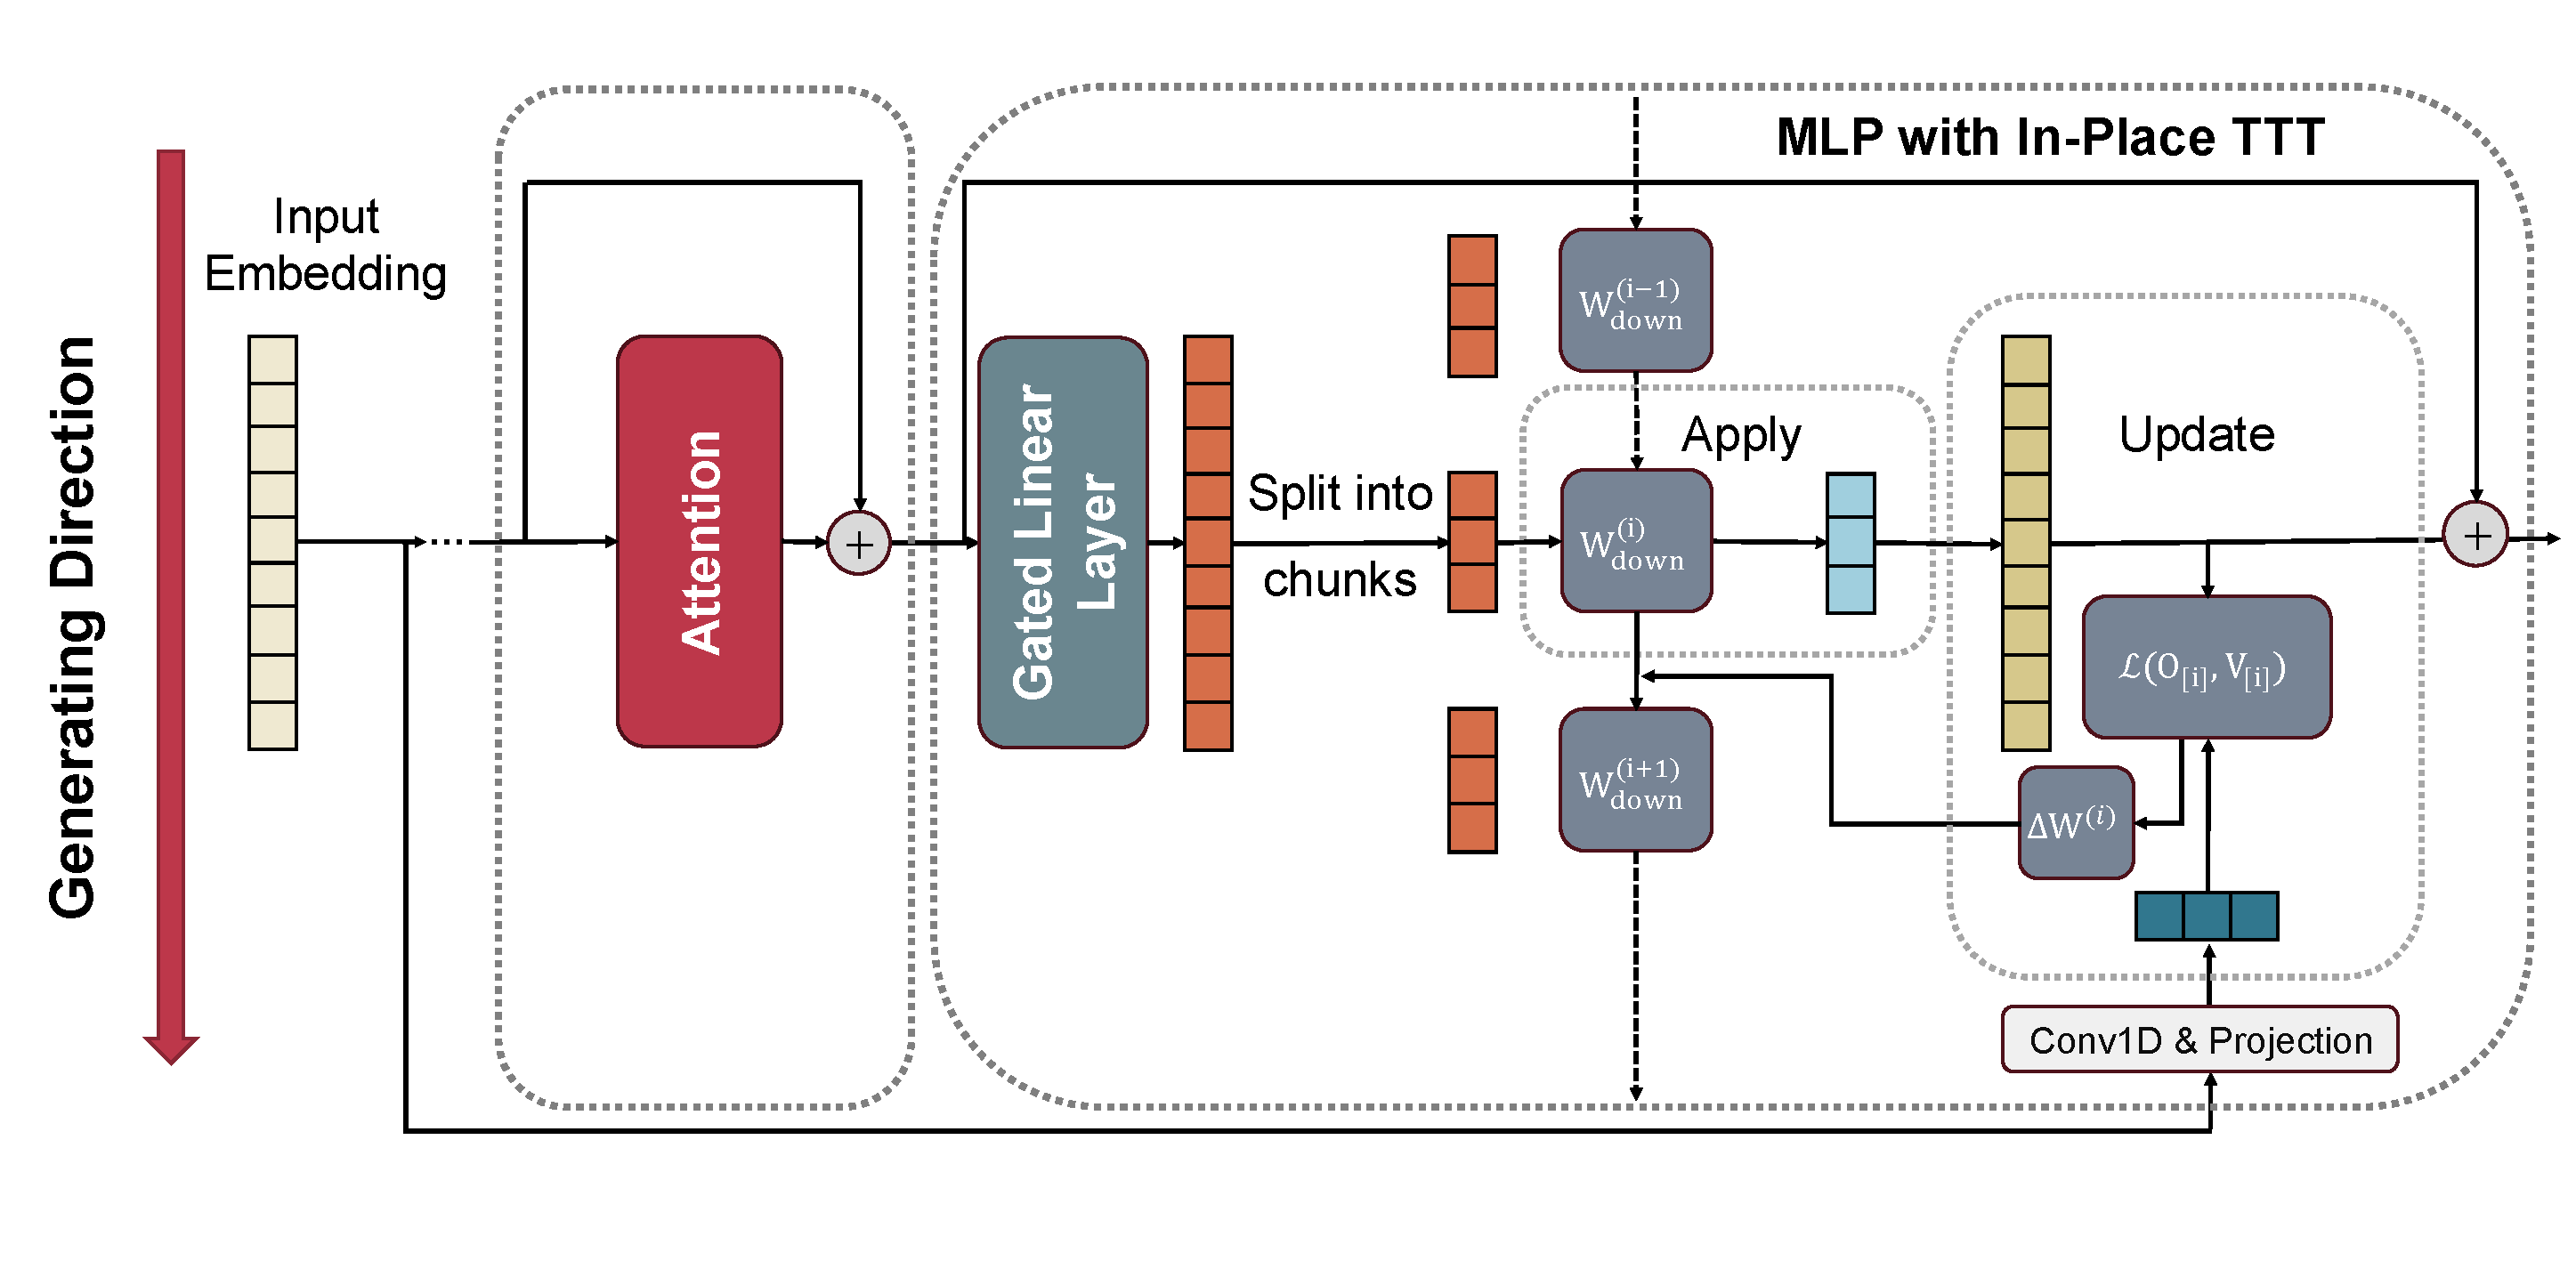
\includegraphics[width=1.0\linewidth]{image/IPTTT.pdf}
    \caption{The overall framework of our In-Place Test-Time Training. The module operates sequentially on input chunks. For each chunk, the current fast weights are first \textit{applied} to the intermediate activations $\mathbf{Z}$ to produce the output. Then, these weights are \textit{updated} using the activations $\mathbf{Z}$ and a value $\mathbf{V}$ derived from the token embeddings. This "apply-then-update" cycle allows the model to dynamically adapt to incoming context in a strictly causal manner.}
    \label{fig:pipeline}
\end{figure}


\subsection{Implementation Details}
\label{sec:implement}


Combining aforementioned designs, \cref{fig:pipeline} illustrates our In-Place TTT framework. Here we further elaborate on practical implementation details, which are engineered for high efficiency and scalability on modern hardware. In particular, our approach is fully compatible with \textit{Context Parallelism (CP)}, relying on a parallel scan algorithm to process sequence chunks simultaneously while preserving the strict causal semantics of an auto-regressive update. Additional discussions are further presented.

\textbf{Efficient Implementation with Context Parallelism.}
The associative nature of our update rule in \cref{eq:final_update_rule} makes In-Place TTT amenable to a context-parallel implementation, which partitions a sequence along its length and processes the chunks simultaneously. The process unfolds into three stages: (\romannumeral1) for all chunks $i \in \{1, \dots, T\}$, we compute the intermediate activations $\mathbf{Z}_{[i]}$ and the fast weight update $\Delta \mathbf{W}_{\mathrm{down}}^{(i)} = (\hat{\mathbf{V}}_{[i]})^\top \mathbf{Z}_{[i]}$ in parallel; (\romannumeral2) a single prefix sum over $[...,\Delta \mathbf{W}_{\mathrm{down}}^{(i)},\Delta \mathbf{W}_{\mathrm{down}}^{(i+1)},...]$ is conducted to compute the aggregated updates for each chunk: $\Delta \mathbf{S}_i = \sum_{j=1}^{i-1} \Delta \mathbf{W}_j$, which can be highly efficient on modern accelerators; (\romannumeral3) the effective fast weights for each chunk, $\mathbf{W}_{\mathrm{down}}^{(i-1)} = \mathbf{W}_{\mathrm{down}}^{(0)} + \eta \Delta\mathbf{S}_i$, and the corresponding output, $\mathbf{O}_{[i]} = \mathbf{Z}_{[i]} (W_{\mathrm{down}}^{(i-1)})^\top$, are computed in parallel.

\textbf{Causality and Boundary Handling.}
To ensure that the update delta for chunk $i$ itself contains no future information, we apply causal padding to the 1D convolution when generating the value. This isolates each delta calculation to its respective chunk, making the parallel scan mathematically equivalent to a sequential update. Moreover, at document boundaries, the fast weights are reset to their pre-trained state to prevent context leakage across independent sequences. The final context parallel algorithm is presented in \cref{alg:inplaceTTT-cp} in Appendix \ref{app:cp}.

\textbf{Discussion.}
In summary, our implementation of In-Place TTT synergistically combines a simple, computationally efficient update rule with a parallel scan algorithm. This design choice makes our method not only fast and scalable but also mathematically equivalent to a strictly causal sequential process, thanks to careful boundary and padding management. The resulting module is \textit{CP-native}, fully causal, and can be seamlessly integrated as a drop-in replacement for the MLP block in standard Transformer architectures. Lastly, it is also noteworthy that the core principles of our framework are orthogonal to the specific choice of loss functions and its optimizer, which have been widely studied in the broader TTT literature, an exploration we leave as a promising direction for future work.